\documentclass{beamer}
%\setbeamercovered{transparent}
%\usepackage{beamerthemesplit}
%\usepackage{movie15}
\usepackage{color,amsmath,xmpmulti,textpos,comment,eurosym,bm,amsthm}

%%%%%%%%%%%%%%%%%%%%%%%%%%%%%%%%%%%%%%%%%%%%%
% Lecture notes preamble
%%%%%%%%%%%%%%%%%%%%%%%%%%%%%%%%%%%%%%%%%%%%%
\input{./../../slides_preamble}

%%%%%%%%%%%%%%%%%%%%%%%%%%%%%%%%%%%%%%%%%%%%%
% LML beamer preamble
%%%%%%%%%%%%%%%%%%%%%%%%%%%%%%%%%%%%%%%%%%%%%
\newenvironment{myindentpar}[1]%
{\begin{list}{}%
    {\setlength{\leftmargin}{#1}}%
  \item[]%
}
{\end{list}}

\usetheme[hideothersubsections]{Hannover}

\newcommand\BackgroundPicture[1]{
\setbeamertemplate{background}{
\parbox[c][\paperheight]{\paperwidth}{
\vfill \hfill
\includegraphics[width=1\paperwidth,height=1\paperheight]{#1}
\hfill \vfill
}}}

\definecolor{lmlblue}{RGB}{0,70,112}
\definecolor{lmlgrey}{RGB}{142,142,142}
\definecolor{grey}{RGB}{210,210,210}

\setbeamercolor{alerted text}{fg=lmlblue}
\setbeamercolor{background canvas}{bg=white}
\setbeamercolor{block body alerted}{fg=lmlblue}
\setbeamercolor{block body}{fg=lmlblue}
\setbeamercolor{block body example}{fg=lmlblue}

\setbeamercolor{block title alerted}{fg=lmlblue}
\setbeamercolor{block title}{fg=lmlblue}
\setbeamercolor{block title example}{fg=lmlblue}

\setbeamercolor{fine separation line}{fg=lmlgrey}
\setbeamercolor{frametitle}{fg=lmlblue}
\setbeamercolor{item projected}{fg=white, bg=lmlblue}
\setbeamercolor{normal text}{fg=black}

\setbeamercolor{palette sidebar primary}{fg=lmlgrey}
\setbeamercolor{palette sidebar quarternary}{fg=lmlgrey}
\setbeamercolor{palette sidebar secondary}{fg=lmlgrey}
\setbeamercolor{palette sidebar tertiary}{fg=lmlgrey}
\setbeamercolor{section in sidebar}{fg=white}
\setbeamercolor{section in sidebar shaded}{fg=grey}

\setbeamercolor{separation line}{fg=lmlgrey}

\setbeamercolor{sidebar}{bg=lmlgrey}
\setbeamercolor{sidebar}{parent=palette primary}

\setbeamercolor{structure}{bg=white, fg=lmlblue}
\setbeamercolor{subsection in sidebar}{fg=white}
\setbeamercolor{subsection in sidebar shaded}{fg=grey}

\setbeamercolor{title}{fg=lmlblue}
\setbeamercolor{titlelike}{fg=lmlgrey}

%%%%%%%%%%%%%%%%%%%%%%%%%%%%%%%%%%%%%%%%%%%%%
% Miscellaneous preamble
%%%%%%%%%%%%%%%%%%%%%%%%%%%%%%%%%%%%%%%%%%%%%
\newcommand{\vs}[1]{\vspace{.#1cm}}
\newcommand{\vf}{\vspace{.25cm}}
\newcommand{\np}{\\ \vf}
\newcommand{\ft}[1]{\frametitle{#1}}

% add frame numbers to navigation bar
% (for RSS 2015 conference)
\addtobeamertemplate{navigation symbols}{}{
    \usebeamerfont{footline}
    \usebeamercolor[fg]{footline}
    \hspace{1em}
    \scriptsize
    \insertframenumber/\inserttotalframenumber
}

\logo{
\includegraphics[width=1.cm]{./figs/lml_square.jpg}}

\title[\insertlogo\\Lecture 2: Decisions]{Lecture 2: Decisions}
\author{Ole Peters\\ Alexander Adamou}
\institute{
\includegraphics[width=4cm]{./figs/lml_LOGO_whiteBG.png}}
\date{SFI Winter School\\ India, 17 December 2015}

\AtBeginSection[]{
\frame{
\ft{Agenda}
\tableofcontents[currentsection]
}
}

%%%%%%%%%%%%%%%%%%%%%%%%%%%%%%%%%%%%%%%%%%%%%
% Document
%%%%%%%%%%%%%%%%%%%%%%%%%%%%%%%%%%%%%%%%%%%%%
\begin{document}

\frame{
\titlepage
}

\frame{
\ft{Agenda}
\tableofcontents
}

\begin{comment}
\end{comment}
%%%%%%%%%%%%%%%%%%%%%%%%%%%%%%%%%%%%%%%%%%%%%
\section{Introduction}

\frame{
\ft{Introduction}
Decision theory as cornerstone of formal economics: models how individuals make decisions.\np
We generalise and formalise treatment of coin tossing game.\np
Axiom: maximise time-average growth rate of wealth.\np
Simple and powerful idea, which removes need for established but epistemologically troublesome techniques.
}

\frame{
\ft{References}
Some of this lecture is based on recent papers (open access):
\bi
\item O.\ Peters and M.\ Gell-Mann. \textit{Evaluating gambles using dynamics.} arXiv:1405.0585, 2014.
\item O.\ Peters. \textit{The time resolution of the St Petersburg paradox.} Phil.\ Trans.\ R.\ Soc. A 369, 4913--4931, 2011.
\item O.\ Peters and A.\ Adamou. \textit{Rational insurance with linear utility and perfect information.} arXiv:1507.04655, 2015.
\ei
}

\frame{
\ft{Models and reality}
Build our decision theory from mathematical model of the gamble problem. Define:
\bi
\item the gamble, a mathematical object; and
\item the decision criterion, a set of instructions containing mathematical manipulations of the gamble.
\ei\mbox{}

Gambles will resemble real-world situations.\np
Criteria may/may not resemble real decision-making.\np
Ignore realism for now: main task is to explore imaginary world of behaviours created by model (like  science fiction).
}

%%%%%%%%%%%%%%%%%%%%%%%%%%%%%%%%%%%%%%%%%%%%%
\section{Gambles}
\frame{
\ft{Gamble}
Gamble as fundamental building block of decision theory.\np
Mathematical object resembling real situation whose outcome:
\bi
\item is purely monetary;
\item is uncertain; and
\item occurs over a specified period of time.
\ei\mbox{} 

Example: buying a lottery ticket.\np
Need formal mathematical definition\ldots
}

\frame{
\ft{Definition}
\begin{defn}{Gamble}
A gamble is a pair of random variable, $\gD$, and duration, $\dt$.\\

$\gD$ is called the payout and takes one of $\N$ possible monetary values, $\{\gD_1,\ldots,\gD_N\}$.\\

Payouts are associated with probabilities, $\{\p_1,\ldots,\p_\N\}$, 

where $\sum_{\gi=1}^\N \p_\gi = 1$.\\

Payouts can be positive, associated with monetary gain, or negative, associated with loss.\\

Order them such that $\gD_1<\ldots<\gD_\N$.
\end{defn}
}

\frame{
\ft{Examples}
\underline{Betting on a fair coin}\np
Imagine betting $\$ 10$ on the toss of a fair coin.\np
Model with payouts and probabilities:
\bea
\gD_1 = -\$ 10, &\quad& \p_1 = 1/2;\\
\gD_2 = +\$ 10, &\quad& \p_2 = 1/2.
\eea
Duration: $\dt=2$ seconds.
}

\frame{
\ft{Examples}
\underline{Playing the lottery}\np
Imagine a lottery, where individual pays $\F$ for a ticket which will win jackpot, $\J$, with probability, $\p$.\np
Payouts and probabilities are:
\bea
\gD_1 = -\F,  &\quad& \p_1 = 1-\p;\\
\gD_2 = \J-\F, &\quad& \p_2 = \p.
\eea
Duration: $\dt=1$ week.
}

\frame{
\ft{Examples}
\only<1>{
\underline{Betting at fixed odds}\np
Imagine a bet placed at fixed odds, \eg on a horse race.\np 
Bet $\F$ on \textit{Ito} to win the Prix de l'Arc de Triomphe at Longchamp at odds of 50/1.\np 
\textit{Ito} will win the race with unknown probability, $\p$.\np
Payouts and probabilities are:
\bea
\gD_1 = -\F,  &\quad& \p_1 = 1-\p;\\
\gD_2 = 50\F, &\quad& \p_2 = \p.
\eea
Duration: $\dt=30$ minutes.
}
\only<2>{
\textit{Ito} did not win. (He didn't even run!)\np
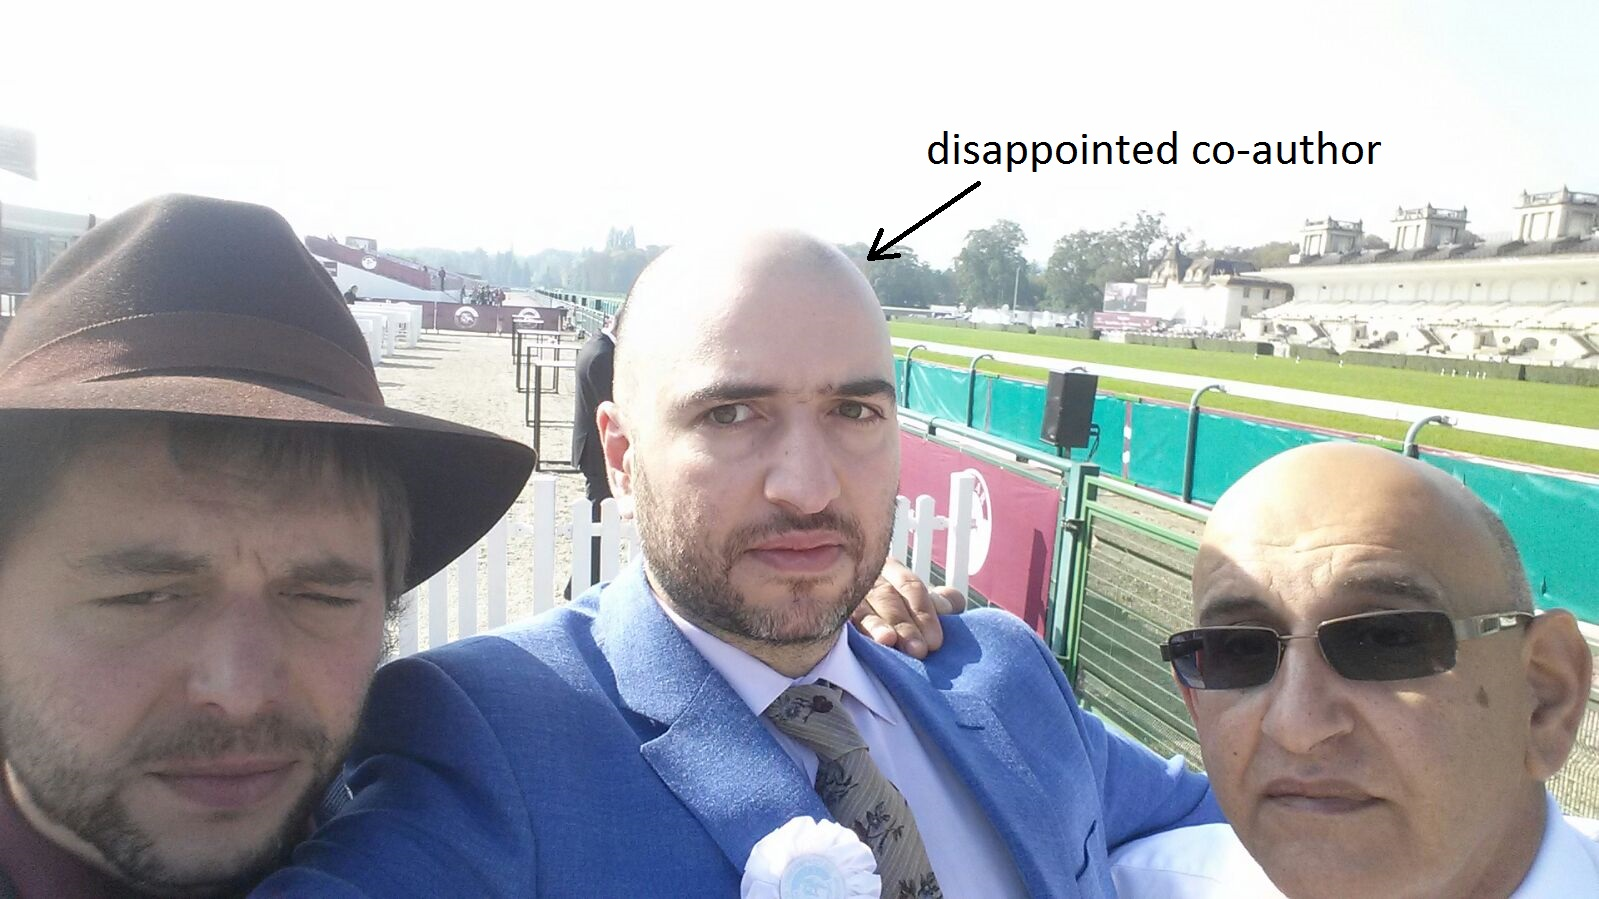
\includegraphics[width=\textwidth]{./figs/longchamp.jpg}
}
}
\frame{
\ft{The null gamble}
Another example is the null gamble, in which a payout of zero is received with certainty:
\be
\gD_1=\$0, \quad \p_1=1.
\ee
Useful for our theory as it represents the `no bet' or `do nothing' option.\np
Duration, $\dt$, must be chosen appropriately (often by reference to an alternative gamble).
}

\frame{
\ft{Discrete and continuous gambles}
Gamble as simple but versatile model of uncertain future.\np
Used to model traditional wagers and other economic activities, \eg stock market investments, insurance contracts, derivatives.\np
We presented discrete gamble, where payout has countable (usually small) number of possible outcomes.\np
Extension to continuous gambles is natural.\np
Used to model real-world scenarios with large number of possible outcomes, \eg change in stock price.
}

\frame{
\ft{The gamble problem}
Suppose you must choose between two scenarios modelled as gambles (possibly including the null gamble).\np
\begin{keypts}{Question}
Which should you choose, and why?
\end{keypts}\mbox{}

This is the gamble problem.\np
Central question in decision theory and basis for most of mainstream economics.
}

%%%%%%%%%%%%%%%%%%%%%%%%%%%%%%%%%%%%%%%%%%%%%
\section{Repetition}

\frame{
\ft{Single gamble}
Gambles are mathematical abstractions, not yet connected to our model humans.\np
Relevant to people only in that they affect wealth process, $\x(\t)$.\np 
Single round in isolation (``one-shot game'') uninstructive: says only that $\x(\t+\dt)=\x(\t)+\gD$, a random variable.\np 
Tendency of $\x(\t)$ over time unclear as one time-step not enough for tendency to emerge.\np
Time has no significance in one-shot game. Value of $\dt$ irrelevant to analysis: could be heartbeat or life of universe!
}

\frame{
\ft{Repeated gambles}
Model wealth evolution by repeating gamble over many rounds.\np
We don't believe real-world situations repeat themselves, \eg we don't have to keep betting on \textit{Ito} (thankfully!)\np
Modelling device to extract otherwise invisible tendencies, reflects idea that consequences of decisions unfold over time.\np
Mode of repetition \textbf{not} specified in gamble: separate model component which must be specified.\np
Focus on two modes: \textbf{additive} and \textbf{multiplicative} repetition.
}

\frame{
\ft{Additive repetition}
\begin{defn}{Additive repetition}
Define change in wealth over single round of gamble as
\be
\d \x(\t) \equiv \x(\t+\dt)-\x(\t).
\elabel{DW_def}
\ee
To repeat additively, simply add random payout to wealth at each round, \ie
\be
\d\x(\t) = \gD.
\elabel{DW_add}
\ee
Note that $\d \x$ is a stationary random variable.
\end{defn}
}

\frame{
\ft{Wealth evolution}
Starting at time $\tn$, wealth after $\T$ rounds is
\be
\x(\tn+\T\dt) = \x(\tn) + \sum_{\gtau=1}^\T \gD(\gtau),
\elabel{Wt_add}
\ee
where $\gD(\gtau)$ is realised payout in round $\gtau$.\np
Evolution equation for wealth following noisy additive dynamic.\np 
Note that $\x(\tn+\T\dt)$ is itself a random variable.
}

\frame{
\ft{Example}
\underline{Additive coin toss}\np
Return to first example gamble: $\$ 10$ fair coin toss.\np
Successive bets always $\$ 10$, regardless of wealth.\np
Suppose $\x(\t_0)=\$ 100$, then wealth after $\T$ rounds is
\bea
\x(\t_0+\T\dt) &=& \$ 100 + \$ 10 \gk - \$ 10 (\T-\gk)\\
&=& \$ [100 +  10(2\gk-\T)],
\eea
where $0\leq \gk\leq \T$ is the number of winning tosses.\np
Note: wealth can go negative (no bankruptcy).
}

\frame{
\ft{Multiplicative repetition}
\only<1>{
An alternative is multiplicative repetition.\np
In example, imagine first $\$ 10$ bet not as fixed size but instead as fixed fraction (10\%) of starting wealth ($\$ 100$).\np
Successive bets are for same fraction of wealth, but different monetary amounts.\np
Formalise as follows\ldots
}
\only<2>{
\begin{defn}{Multiplicative repetition}
Express payout, $\gD$, in first round as random wealth multiplier:
\be
\gr \equiv \frac{\x(\t_0)+\gD}{\x(\t_0)}.
\elabel{R_def}
\ee
Repeat gamble by applying multiplier at subsequent rounds:
\be
\x(\t+\dt) = \gr\x(\t).
\ee
\end{defn}
}
}

\frame{
\ft{Wealth evolution}
$\gr$ is a stationary random variable but change in wealth,
\be
\d \x(\t) = (\gr-1)\x(\t),
\elabel{DW_mult_short}
\ee
depends on $\t$ through $\x(\t)$.\np
Wealth after $\T$ rounds of gamble is
\be
\x(\t_0+\T\dt) = \x(\t_0)\prod_{\gtau=1}^\T \gr(\gtau),
\ee
where $\gr(\gtau)$ is realised multiplier in round $\gtau$.
}

\frame{
\ft{Example}
\underline{Multiplicative coin toss}\np
Repeat $\$10$ coin toss multiplicatively.\np
Random multiplier, $\gr$, has two possible possible outcomes:
\bea
\gr_1 = \frac{\$100 - \$10}{\$100} = 0.9, &\quad& \p_1 = 1/2;\\
\gr_2 = \frac{\$100 + \$10}{\$100} = 1.1, &\quad& \p_2 = 1/2.
\eea
Wealth after $\T$ rounds with $\gk$ winning tosses:
\be
\x(\t_0+\T\dt) = \$100\,\,(1.1)^\gk\,(0.9)^{\T-\gk}.
\ee
Note: no possibility of negative wealth or bankruptcy, since individual can lose at most 10\% of wealth in a round.
}

\frame{
\ft{Choose appropriate dynamic}
Imagined mode of repetition not simply matter of taste.\np
Consequence of choice is huge: additive and multiplicative dynamics differ as starkly as linear and exponential functions.\np
Therefore must consider economic situation to be modelled and choose realistic dynamic.\np
\eg Stock price fluctuations tend to be $\propto$ price $\to$ appropriate dynamic is multiplicative.
}

%%%%%%%%%%%%%%%%%%%%%%%%%%%%%%%%%%%%%%%%%%%%%
\section{Growth rates}

\frame{
\ft{Growth rates}
We have linked $\x(\t)$ to the gamble \textit{via} a dynamic.\np
Can now develop decision criterion.\np
Good advice: ``Pick the gamble that will cause your wealth to grow fastest.''\np
To formalise this we need to revisit growth rates.
}

\frame{
\ft{Stationarity}
Previously introduced growth rate, $\g$, as rate of change of strictly increasing function, $\gv(\x)$:
\be
\g(\t,\Dt) \equiv \frac{\D \gv(\x(\t))}{\Dt}.
\elabel{g_def}
\ee
$\gv(\x)$ chosen so that increment, $\D \gv(\x(\t))$, over general time period, $\Dt$, is stationary random variable.\np
$\to$ $\g(\t,\Dt)$ also stationary: \textit{distribution} independent of $t$.\np
Stationarity (\ie statistical irrelevance of measurement time) is crucial $\to$ want distribution of $\g$ to convey robust information about wealth process, not merely when it was sampled.
}

\frame{
\ft{Additive growth rate}
Additive repetition: $\D\x$ already stationary.\np
$\to$ Appropriate mapping is $\gv(\x)=\x$.\np
$\to$ Growth rate under additive repetition is
\be
\g_\text{a}(\t,\Dt) = \frac{\D\x(\t)}{\Dt}.
\elabel{g_add}
\ee
}

\frame{
\ft{Multiplicative growth rate}
Multiplicative repetition: $\D\x$ not stationary $\to$ need mapping $\gv(\x)$ with stationary increment. Note that over one round
\bea
\d\ln \x(\t) &=& \ln \x(\t+\d\t) - \ln \x(\t)\\
&=& \ln \gr\x(\t) - \ln \x(\t)\\
&=& \ln \gr,
\eea
which is stationary because $\gr$ is stationary.\np
$\to$ Appropriate mapping is $\gv(\x)=\ln\x$.\np
$\to$ Growth rate under multiplicative repetition is:
\be
\gm(\t,\Dt) = \frac{\D\ln \x(\t)}{\Dt}.
\elabel{g_mult}
\ee
}

\frame{
\ft{Time-average growth rate}
Distribution of $\g(\t,\Dt)$ depends on $\Dt$.\np
In general, distribution narrows as $\Dt$ increases, converging to a finite number as $\Dt\to\infty$.\np
Repetition over long time exposes tendency of gamble.
\begin{defn}{Time-average growth rate}
Define time-average growth rate as
\be
\gt \equiv \lim_{\Dt\to\infty}\{\g(\t,\Dt)\}.
\ee
\end{defn}
}

\frame{
\ft{Ergodicity}
$\gt$ is growth rate over diverging rounds of gamble:
\be
\gt = \lim_{\T\to\infty} \left\{ \frac{ \gv(\x(\t+\T\dt)) - \gv(\x(\t)) }{\T\dt } \right\}.
\ee
Expand numerator as sum of single-round increments:
\bea
\gt &=& \lim_{\T\to\infty} \left\{ \frac{1}{\T} \sum_{\gtau=1}^\T \frac{ \D \gv(\x(\t+\gtau\dt)) }{ \dt } \right\} \\
&=& \lim_{\T\to\infty} \left\{ \frac{1}{\T} \sum_{\gtau=1}^\T \g(\t+\gtau\dt,\dt) \right\} \;=\; \ave{\g(\t,\dt)}
\eea
by stationarity and independence of successive growth rates.\np
Restatement of ergodic property: time and ensemble averages of ergodic growth rate have same value.
}

\frame{
\ft{Ergodic growth rates}
Equivalences for additive and multiplicative dynamics:
\bea
\gt_\text{a} &=& \lim_{\Dt\to\infty}\left\{\frac{\D\x(\t)}{\Dt}\right\} = \ave{\frac{\D\x(\t)}{\Dt}}; \elabel{g_bar_a}\\
\gt_\text{m} &=& \lim_{\Dt\to\infty}\left\{\frac{\D\ln \x(\t)}{\Dt}\right\} = \ave{\frac{\D\ln \x(\t)}{\Dt}}. \elabel{g_bar_m}
\eea
General equivalence:
\be
\gt = \lim_{\Dt\to\infty}\left\{\frac{\D \gv(\x(\t))}{\Dt}\right\} = \ave{\frac{\D \gv(\x(\t))}{\Dt}}. \elabel{g_bar_gen}
\ee 
Value of $\Dt$ in $\ave{\ }$ immaterial. Gamble duration, $\dt$, often used.\np
No special interpretation of $\ave{\g}$. Just happens to coincide with quantity of interest, $\gt$.
}

\frame{
\ft{Scalars}
\only<1>{
General remarks on story so far.\np
Start with high-dimensional mathematical object: gamble.\np
Add dynamic: instructions for how wealth evolves when gamble repeated.\np
Collapse this information to a scalar (single number), $\gt$, which summarises effect of gamble on wealth.\np
Scalars can be ranked unequivocally $\to$ clear decision criterion.\np
Hard to devise for high-dimensional objects, \eg return distributions\ldots
}
\only<2>{

\centering
Blue or red?\\
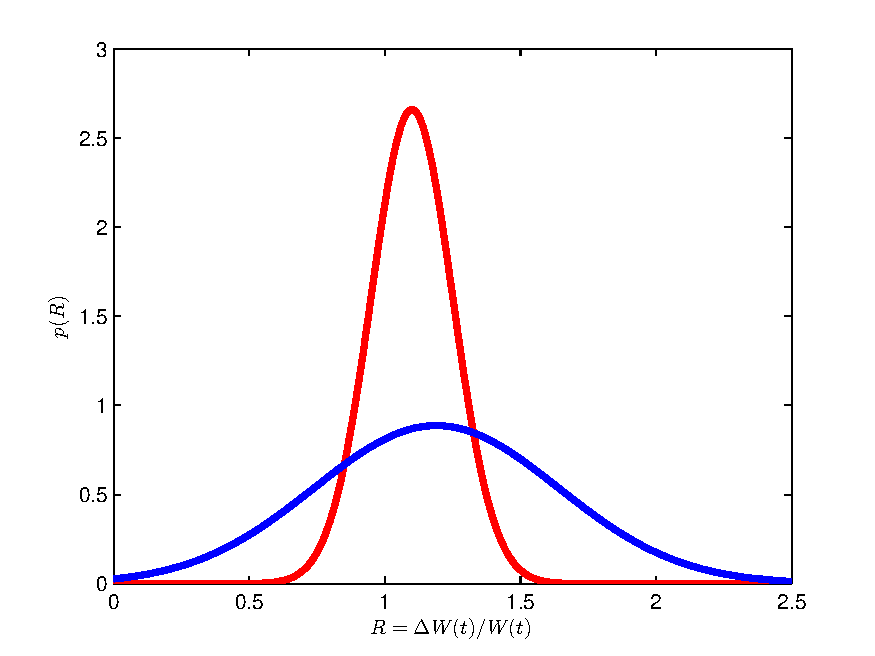
\includegraphics[width=0.9\textwidth]{./figs/dec_dist.pdf}
}
}

%%%%%%%%%%%%%%%%%%%%%%%%%%%%%%%%%%%%%%%%%%%%%
\section{Decision axiom}

\frame{
\ft{Model rationale}
Model rationale for deciding between gambles: maximise $\gt$ for the specified mode of repetition.\np
In other words, model humans choose gamble which, if repeated indefinitely, causes wealth to grow fastest.\np
Indefinite repetition as conceptual device or thought experiment to elicit tendency of gamble.\np
In real world a particular choice between gambles may only occur once.\np
But also true that real decisions followed by many others.
}

\frame{
\ft{Plausibility and parsimony}
In model this decision rule outperforms all others in the long run $\to$ plausible logical basis.\np
Where model approximates real world, expect rationale to approximate real decisions.\np 
Rationale is parsimonious, based on a single robust quantity derived from minimal model components (gamble, dynamic).\np
No arbitrary or unquantifiable human psychological factors.
}

\frame{
\ft{Axiom}
Nevertheless, decision criterion has status of \textit{axiom}: it is asserted as premise of model.\np
Generates model world where certain behaviours observed.\np
Hope is for model world to resemble real world, but you may disagree.\np
Other decision axioms possible, \eg classical decision theory based on axiom that humans maximise expected utility.
}

\frame{
\ft{Algorithm}
\only<1>{
Decision criterion expressible as set of instructions.\np
Denote by $\mbox{}^{(\m)}$ quantities relating to $\m^\text{th}$ available gamble.\np
Each gamble specified by:
\bi
\item random payout, $\gD^{(\m)}$; and
\item duration, $\dt^{(\m)}$.
\ei\mbox{}

Common dynamic for all gambles.
}
\only<2>{
\begin{keypts}{Growth-optimal decision algorithm}
\begin{enumerate}
\item Specify $\gD^{(\m)}$ and $\dt^{(\m)}$ for gambles offered;
\item Specify wealth dynamic, \ie relationship between $\d\x(\t)$, $\x(\t)$, and $\gD$;
\item Determine function, $\gv(\x)$, whose increments are stationary random variables under dynamic;
\item Determine time-average growth rates, $\gt^{(\m)}$, by taking time or ensemble averages of ergodic growth rates, $\g^{(\m)}(\t,\Dt)$;
\item Choose gamble, $\m$, with the largest $\gt^{(m)}$.
\end{enumerate}
\end{keypts}
}
}

\frame{
\ft{Example setup}
Example decisions are between two gambles, \ie $\m\in\{1,2\}$.\np
Decisions between three or more gambles straightforward extensions.\np
Often one option is the null gamble, which trivially has zero growth rate.\np
Then question posed is whether other gamble preferable to doing nothing, \ie accept or decline?\np
}

\frame{
\ft{Example game}
Apply decision algorithm to original coin toss game.\np
Starting wealth $\x(\tn)>\$ 0$, duration $\dt$, random payout:
\bea
\gD^{(1)}_1 = -0.4\x(\t_0), &\quad& \p^{(1)}_1 = 1/2; \\
\gD^{(1)}_2 = 0.5\x(\t_0), &\quad& \p^{(1)}_2 = 1/2.
\eea
Note that payouts $\gD^{(1)}_\gi$ are fixed monetary amounts, expressed here as fractions of $\x(\t_0)$.\np
Choice is between coin toss game and null gamble:
\be
\gD^{(2)}_1 = \$0, \quad \p^{(2)}_1 = 1.
\ee
Analyse under additive and multiplicative repetition.
}

\frame{
\ft{Example}
\only<1>{
\underline{Additive repeated coin toss}\np
Wealth evolution over $T$ rounds (no bankruptcy):
\bea
\x^{(1)}(t_0+\T\dt) &=& \x(\t_0) + \sum_{\gtau=1}^\T \gD^{(1)}(\gtau); \\
\x^{(2)}(t_0+\T\dt) &=& \x(\t_0).
\eea
$\gv(\x)=\x$, so growth rates per unit time are:
\bea
\g_\text{a}^{(1)}(\t) \;=\; \frac{\x^{(1)}(\t+\T\dt) - \x(\t_0)}{\T\dt} &=& \frac{1}{\T}\sum_{\gtau=1}^\T \frac{\gD^{(1)}(\gtau)}{\dt}; \elabel{g1_add}\\
\g_\text{a}^{(2)}(\t) \;=\; \frac{\x^{(2)}(\t+\T\dt) - \x(\t_0)}{\T\dt} &=& \$ 0.
\eea
}
\only<2>{
Trivially $\gt_\text{a}^{(2)}=\$0$ per unit time. For coin toss,
\bea
\gt_\text{a}^{(1)} &=& \ave{\frac{\gD^{(1)}}{\dt}}\\
&=& \frac{\p^{(1)}_1 \gD^{(1)}_1 + \p^{(1)}_2 \gD^{(1)}_2}{\dt}\\
&=& \frac{\x(\t_0)}{20\dt}
\eea
per unit time. This is positive, so $\gt_\text{a}^{(1)}>\gt_\text{a}^{(2)}$.\np 
\textbf{Individual accepts coin toss under additive dynamics.}
}
}

\frame{
\ft{Realism}
Decision rule under additive repetition is to maximise $\ave{\gD/\dt}$, \ie which is rate of change of expected wealth.\np
This coincides under additive dynamic with time-average growth rate.\np
See later that real people usually don't maximise $\ave{\gD/\dt}$.\np 
No great shock: additive repetition without bankruptcy is hardly most realistic model of wealth evolution.\np
Try multiplicative repetition instead.
}

\frame{
\ft{Example}
\only<1>{
\underline{Multiplicative repeated coin toss}\np
Payout, $\gD^{(1)}$, expressed as per-round multiplier,
\be
\gr^{(1)} = \frac{\x(\t_0)+\gD^{(1)}}{\x(\t_0)},
\ee
with possible values:
\bea
\gr^{(1)}_1 = \frac{\x(\t_0)+\gD^{(1)}_1}{\x(\t_0)} = 0.6, &\quad& \p^{(1)}_1 = 1/2; \\
\gr^{(1)}_2 = \frac{\x(\t_0)+\gD^{(1)}_2}{\x(\t_0)} = 1.5, &\quad& \p^{(1)}_2 = 1/2.
\eea
}
\only<2>{
Wealth evolves according to:
\bea
\x^{(1)}(\t_0+\T\dt) &=& \x(\t_0) \prod_{\gtau=1}^\T \gr^{(1)}(\gtau); \elabel{W1T_mult}\\
\x^{(2)}(\t_0+\T\dt) &=& \x(\t_0).\elabel{W2T_mult}
\eea
}
\only<3>{
$\gv(\x)=\ln\x$ so growth rates per unit time are:
\bea
\g_\text{m}^{(1)}(\t) = \frac{\ln \x^{(1)}(\t+\T\dt) - \ln \x(\t_0)}{\T\dt} &=& \frac{1}{\T}\sum_{\gtau=1}^\T \frac{\ln \gr^{(1)}(\gtau)}{\dt}; \elabel{g1_add}\\
\g_\text{m}^{(2)}(\t) = \frac{\ln \x^{(2)}(\t+T\dt) - \ln \x(\t_0)}{\T\dt} &=& 0
\eea
Trivially $\gt_\text{m}^{(2)}=0$ per unit time. For the coin toss,
\bea
\gt_\text{m}^{(1)} = \ave{\frac{\ln \gr^{(1)}}{\dt}} = \frac{\ln0.9}{2\dt},
\eea
per unit time. This is negative, so $\gt_\text{m}^{(1)}<\gt_\text{m}^{(2)}$.\np
\textbf{Decline coin toss under multiplicative dynamics.}
}
}

\frame{
\ft{Warning}
Decision rule under multiplicative repetition is to maximise
\be
\ave{\frac{\ln \gr}{\dt}} = \ave{\frac{\ln(\x(\t_0)+\gD)-\ln \x(\t_0)}{\dt}},
\ee
which coincides with the time-average growth rate.\np
For choice of gambles in example, get \textit{opposite} of decision under additive repetition.\np
$\to$ Realistic dynamic crucial for modelling real decisions.\np
Inappropriate dynamic could lead to very bad advice!\np
}

\frame{
\ft{Alternative presentation}
\only<1>{
Can also present multiplicative repetition without the logarithmic mapping.\np
Wealth after $\T$ rounds (with $\gk$ winning tosses) is
\be
\x^{(1)}(\t_0+\T\dt) = \x(\t_0)\left(\gr_\T^{(1)}\right)^\T,
\ee
where
\be
\gr_\T^{(1)} = (0.6)^{(\T-\gk)/\T}(1.5)^{\gk/\T}
\ee
is the equivalent per-round multiplier.
}
\only<2>{
$\gr_\T^{(1)}$ is a random variable but it converges to
\be
\gr_\infty^{(1)} \equiv \lim_{\T\to\infty}\left\{\gr_\T^{(1)}\right\} = (0.6)^{1/2}(1.5)^{1/2} = \sqrt{0.9},
\ee
since $\gk/\T\to1/2$ as $\T\to\infty$ (fair coin).\np
$\gr_\infty^{(1)}<1$ so wealth decays over time $\to$ coin toss declined.\np
Approaches are linked in that
\be
\gt_\text{m}^{(1)} = \frac{\ln \gr_\infty^{(1)}}{\dt}.
\ee
}
}

%%%%%%%%%%%%%%%%%%%%%%%%%%%%%%%%%%%%%%%%%%%%%
\section{Classical theory}

\frame{
\ft{Expected-wealth paradigm}
Our decision rule under additive repetition is to maximise
\be
\ave{\frac{\D\x}{\Dt}} = \ave{\frac{\d\x}{\dt}} = \ave{\frac{\gD}{\dt}},
\elabel{ex_crit}
\ee
\ie rate of change of expectation value of wealth.\np
``Expected-wealth paradigm'' of $17^\text{th}$ century.\np  
Axiom -- not derived from dynamics or other considerations.\np
Simple rule, familiar average, incorporates gamble outcomes.\np
Has logical basis if game played many times in parallel to access multiple outcomes.
}

\frame{
\ft{Risk neutrality}
In language of economics, expected-wealth paradigm treats humans as ``risk neutral''.\np
\ie No preference between gambles with equal changes in expected wealth over equal duration.\np
For example, fair coin toss at even odds same as doing nothing.\np
Recognised as unrealistic model since at least 1713, as predictions contradicted by observed human behaviour.
}

\frame{
\ft{Predictive failure -- a fix}
Conventional reason for predictive failure is that value assigned by humans to possible changes in wealth depends on:
\bi
\item existing wealth; and
\item psychological risk preferences.
\ei\mbox{}

\ie People don't treat equal amounts of money equally.\np
Makes intuitive sense:
\bi
\item $\D\x=\$10$ more significant to poor than to rich;
\item some people gamble recreationally, others don't.
\ei
}

\frame{
\ft{Expected-utility paradigm}
D.\ Bernoulli 1738 built ideas into ``expected-utility paradigm''.\np
Observation: usefulness of $\Dx$ not linear in $\Dx$.\np
Model: individual has idiosyncratic utility function, $\gu(\x)$, mapping wealth, $\x$, to usefulness, $\gu$.\np
Claim: $\gu$ is quantity whose rate of change of expected value,
\be
\ave{\gr_\gu} \equiv \ave{\frac{\D\gu(\x)}{\Dt}},
\elabel{euh}
\ee
is maximised in a decision between gambles.\np
Axiom of utility theory $\to$ alternative decision algorithm\ldots
}

\frame{
\ft{Algorithm}
\begin{keypts}{Expected-utility decision algorithm}
\begin{enumerate}
\item Specify $\gD^{(\m)}$ and $\dt^{(\m)}$ for gambles offered;
\item Specify idiosyncratic utility function, $\gu(\x)$, which maps wealth to utility;
\item Determine rate of change of expected utility, \eg over single round of gamble,
\be
\ave{\gr_\gu}^{(\m)}=\ave{\frac{\gu\left(\x+\gD^{(\m)}\right)-\gu(\x)}{\dt^{(\m)}}};
\ee
\item Choose gamble, $\m$, with largest $\ave{\gr_\gu}^{(\m)}$.
\end{enumerate}
\end{keypts}
}

\frame{
\ft{Equivalent approaches}
Our decision theory and mainstream utility theory have different conceptual foundations but similar maximands:
\be
\gt = \ave{\frac{\D\gv(\x)}{\Dt}}; \quad \ave{\gr_\gu} = \ave{\frac{\D\gu(\x)}{\Dt}}.
\ee
Stationarity mapping, $\gv(\x)$, depends on wealth dynamic.\np
Utility function, $\gu(\x)$, depends on psychological attitude to risk.\np
Approaches mathematically equivalent if we identify $\gv$ with $\gu$.\np
But suspect debates easier to settle empirically for dynamic than for psychology $\to$ better science.\np
}

\frame{
\ft{Discussion}
Utility theory consistent with $\gt$ maximisation for matching pairs of dynamic and utility function.\np 
But utility theory is a poorly constrained model, because infinitely many admissible $\gu$ and, therefore, $\ave{\gr_\gu}$.\np
Our approach requires dynamic to be specified $\to$ unique $\gv$, $\gt$.\np
$\gv=\ln\x$ for multiplicative repetition.\np
$\gu=\ln\x$ most widely used utility function.\np
Coincidence? Or humans evolved to make growth-optimal decisions in multiplicative environments?
}

\frame{
\ft{Predictive failure -- reason}
Suggests different, deeper reason for predictive failure of expected-wealth paradigm.\np
Good model of decisions under additive repetition.\np
But additivity poor model of wealth evolution (\eg bank interest payments independent of balance).\np 
Fails to predict reality because implicitly contains unrealistic dynamic. 
}


%%%%%%%%%%%%%%%%%%%%%%%%%%%%%%%%%%%%%%%%%%%%%
\section{St Petersburg paradox}

\frame{
\ft{Background}
Devised by N.\ Bernoulli 1713 to test expected-wealth paradigm as model of human decision-making.\np
Hypothetical lottery with diverging rate of change of expected wealth for any ticket price.\np
Expected-wealth paradigm predicts people will pay any price.\np
Paradox: people observed to want to wager only small sums.\np
Motivation for development of expected-utility paradigm.
}

\frame{
\ft{An unhelpful problem}
Lottery deliberately provocative and unrealistic.\np
No need to invent gamble with $\ave{\d\x}\to\infty$ to expose flaws in expected-wealth paradigm.\np
Divergences in problem and proposed solutions confusing and allow non-fundamental objections of physical impossibility.\np
Such objections address only specific gamble, not paradigm.\np
But indelible part of history and current mainstream theory.
}

\frame{
\ft{St Petersburg lottery}
\only<1>{
Traditional statement of lottery as follows:\np
Imagine starting prize of $\$1$ (originally ducats).\np
Toss a coin:
\bi
\item if heads, prize is won and lottery ends;
\item if tails, prize is doubled and the process is repeated.
\ei\mbox{}

Prize is $\$2$, $\$4$, $\$8$ if first head on $2^\text{nd}$, $3^\text{rd}$, $4^\text{th}$ toss, \etc\np 
Player pays $\F$ for lottery ticket.\np
Question: what is largest $\F$ they are willing to pay?
}
\only<2>{
Lottery translates neatly into our gamble formalism:
\be
\gD_\gk = \$ 2^{\gk-1} - \F, \quad \p_\gk = 2^{-\gk},
\elabel{lottery_def}
\ee
for $\gk\in\{1,2,3,\ldots\}$, \ie set of positive integers.\np
Vast majority of \textit{observed} payouts are small, but rarely extremely large payouts occur.\np
See simulated trajectories with lottery repeated additively.
}
}

\frame{
\ft{Additive simulation}
\centering
10 trajectories, 1000 rounds, $\x(0)=\$100$, $\F=\$10$.
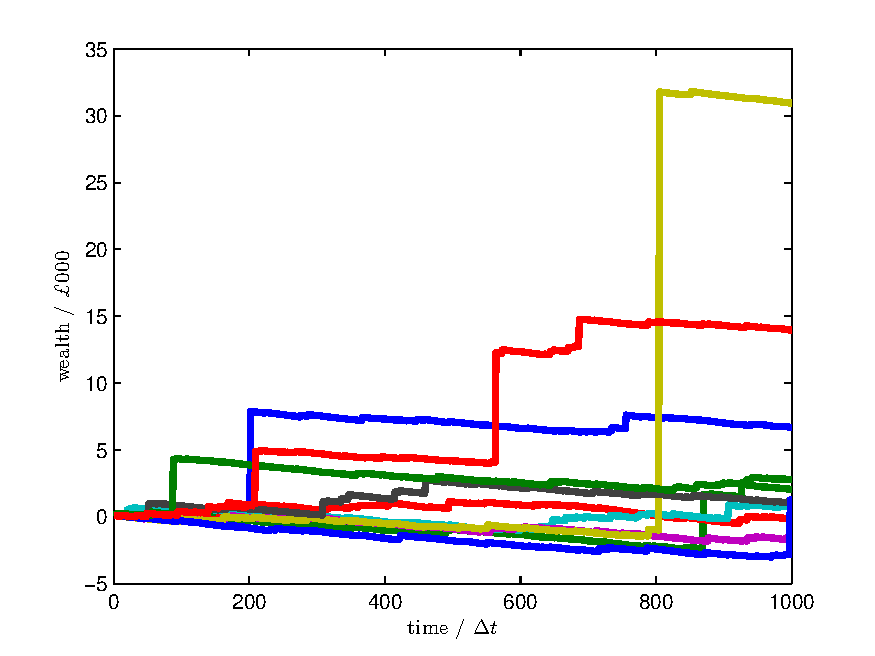
\includegraphics[width=0.9\textwidth]{./figs/lottery_add_traj.pdf}
}

\frame{
\ft{Paradox}
\only<1>{
Coin tosses simply mechanism for selecting outcome $\to$ ignore.\np
Use compact definition of lottery and assume duration $\dt$.\np
Rate of change of expected wealth:
\bea
\frac{\ave{\d\x}}{\dt} & = & \frac{1}{\dt} \sum_{\gk=1}^\infty \p_\gk \gD_\gk \\
&=& \frac{1}{\dt} \left( \$ \sum_{\gk=1}^\infty 2^{-\gk}\,2^{\gk-1} - \sum_{\gk=1}^\infty 2^{-\gk} \F \right) \\
&=& \frac{1}{\dt} \left( \$ \sum_{\gk=1}^\infty \frac{1}{2} - \F \right) \;\to\; \infty \quad \text{\underline{for all $\F$}}.
\elabel{lottery_ex_wealth}
\eea
Expected-wealth paradigm: lottery favourable at \textit{any} price -- including one's entire wealth!
}
\only<2>{
\textit{Reductio ad absurdum}: real people do not behave this way.\np
D.\ Bernoulli resolved paradox using utility function, $\gu(\x)=\ln \x$.\np
(Equivalent to maximising $\gtm$ under multiplicative repetition.)\np 
Bernoulli made a mathematical error implementing his own paradigm.\np
We focus on what we presume he meant to write\ldots
}
}

\frame{
\ft{Resolution by logarithmic utility}
\only<1>{
Rate of change of expected logarithmic utility,
\bea
\frac{\ave{\d\ln \x}}{\dt} & = & \frac{1}{\dt} \sum_{\gk=1}^\infty \p_\gk \left[\ln(\x+\gD_\gk)-\ln \x\right] \\
&=& \frac{1}{\dt} \sum_{\gk=1}^\infty 2^{-\gk} \ln\left(\frac{\x+\$2^{\gk-1}-\F}{\x}\right), \elabel{lottery_ex_util}
\eea
where $\x$ is the ticket buyer's wealth.\np
Finite for ticket price less than wealth plus booby prize: $\F<\x+\$1$ (\ie price that prevents bankruptcy).\np
In particular, $\ave{\d\ln\x/\dt}$ can be positive or \textit{negative} $\to$ lottery can be declined in favour of null gamble.
}
\only<2>{
\centering
Locus in $(\x,\F)$-plane with $\ave{\d\ln\x/\dt}=0$.
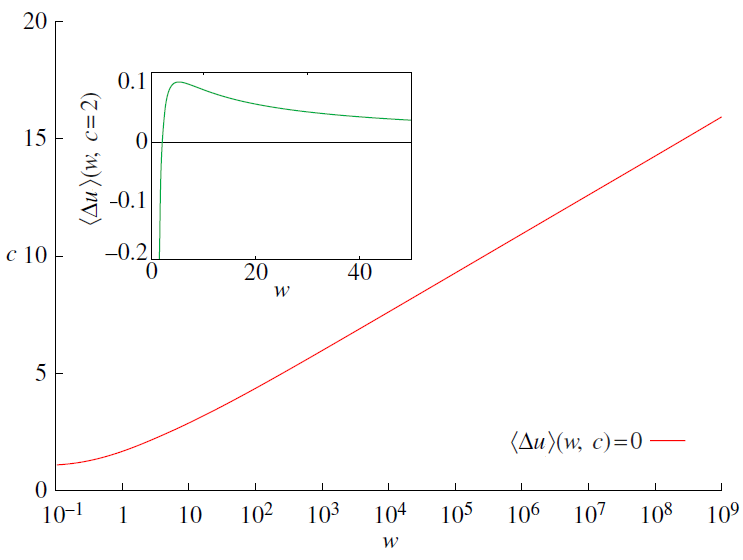
\includegraphics[width=0.9\textwidth]{./figs/gbar_zero.png}
}
\only<3>{
Bernoulli argued plausibly for this resolution: usefulness of monetary gain depends on how much money already have.\np
Also argued plausibly for logarithm: gain in usefulness proportional to fractional gain in wealth: $\gd\gu = \gd\x/\x$.\np
Did not connect to repetition over time (or would have been less willing to accept Cramer's $\gu=\sqrt{\x}$).
}
}

\frame{
\ft{Time resolution}
\only<1>{
Resolve using our decision algorithm.\np
Assume lottery repeated multiplicatively: in effect, prizes and ticket price treated as fractions of player's wealth.\np
Get random wealth multiplier at each round:
\be
\gr_\gk = \frac{\x+\$2^{\gk-1}-\F}{\x}, \quad \p_\gk = 2^{-\gk}.
\ee
Follows earlier treatment of multiplicative gamble $\to$ apply results directly.
}
\only<2>{
Time-average growth rate is
\be
\gt_\text{m} = \frac{1}{\dt} \lim_{\T\to\infty} \left\{ \frac{1}{\T}  \sum_{\gtau=1}^\T \ln \gr(\gtau) \right\} = \frac{1}{\dt}  \sum_{\gk=1}^\infty 2^{-\gk} \ln \gr_\gk, \elabel{lottery_gbar}
\ee
identical to rate of change of expected log-utility.\np
(Because $\gt_\text{m}$ is the ergodic growth rate for multiplicative dynamics.)\np
Same result, different interpretation, fewer assumptions.
}
\only<3>{
Plotted locus marks the decision threshold \textit{vs.}\ null gamble under our decision rule.\np
Player can sensibly decline the gamble $\to$ paradox resolved.\np
Can simulate trajectories for multiplicative repetition of same lotteries that we previously repeated additively.\np
Visualise decaying tendency in a realistic dynamic.
}
}

\frame{
\ft{Multiplicative simulation}
\centering
10 trajectories, 1000 rounds, $\x(0)=\$100$, $\F=\$10$.
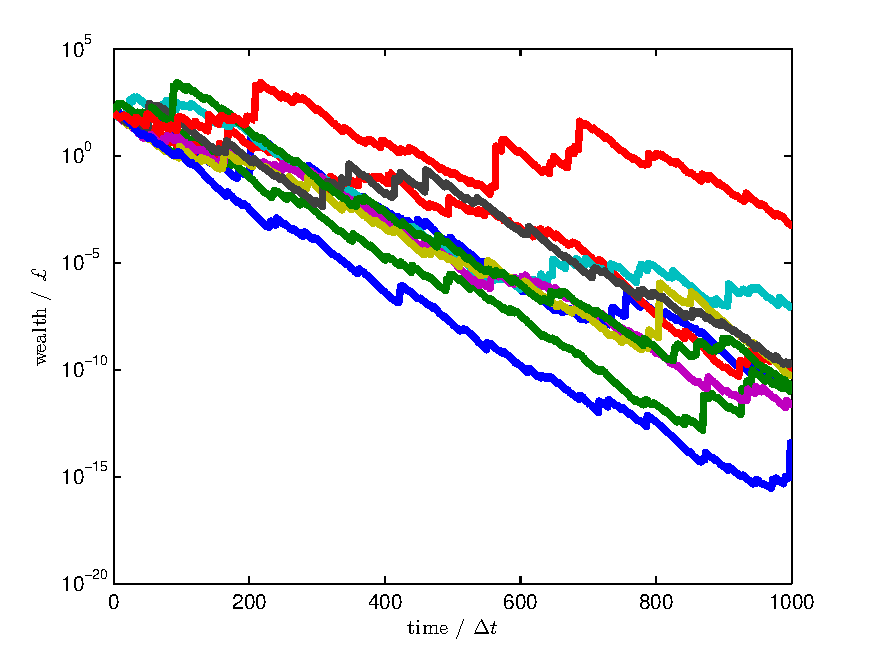
\includegraphics[width=0.9\textwidth]{./figs/lottery_mult_traj.pdf}
}

\frame{
\ft{Discussion}
Treatments based on multiplicative repetition have appeared sporadically in the literature:
\bi
\item explicitly by Whitworth 1870 (in appendix of textbook);
\item related to \Ito's lemma 1944;
\item related to Kelly criterion 1956;
\item explicitly by Cover \& Thomas 1991 (again in textbook);
\item rigorous treatment by Peters 2011.
\ei\mbox{}

Mainstream economics has ignored these.\np
Paradox remains a classic example and a topic of debate.
}

%%%%%%%%%%%%%%%%%%%%%%%%%%%%%%%%%%%%%%%%%%%%%
\section{Insurance}

\frame{
\ft{Background}
Insurance important and ubiquitous economic transaction, which can be modelled as gamble.\np
But in expected-wealth paradigm, buying insurance only rational at prices at which irrational to sell:
\begin{enumerate}
\item To be viable, insurer must charge at least expected value of possible claims (``net 
premium'').
\item So buyer must be willing to pay more than net premium.
\item In expected-wealth paradigm, buyer should decline contract priced at more than 
net premium.
\item Therefore insurance contracts should not exist.
\end{enumerate}
}

\frame{
\ft{Puzzle}
In this picture, insurance only ever beneficial to one party.\np
Anti-symmetry: expected value of one side's gain = expected value of other side's loss.\np
Puzzle: insurance contracts are observed to exist. Why?\np
Classical resolutions: utility theory (\ie psychology) and asymmetric information (\ie deception).\np New resolution: contracts exist with range of prices that increase $\gtm$ for both buyer and seller.\np
Illustrate with example from maritime trade\ldots
}

\frame{
\ft{Model shipping contract}
Imagine shipowner sends cargo St Petersburg $\to$ Amsterdam:
\bi
\item owner's wealth, $\x_\text{own}=\$100,000$;
\item gain on safe arrival of cargo, $\G=\$4,000$;
\item probability ship will be lost, $\p=0.05$;
\item replacement cost of the ship, $\C=\$30,000$;
\item voyage time, $\dt=1$ month.
\ei\mbox{}

Insurer with wealth $\x_\text{ins}=\$1,000,000$ offers to insure voyage for fee, $\F=\$1,800$.\np
If ship lost, insurer pays $\gL=\G+\C$ for ship and lost profit.
}

\frame{
\ft{Owner's gamble}
Frame owner's decision as choice between two gambles. 
\begin{defn}{Owner's decision}
Sending the ship uninsured is gamble o1:
\bea
\gD_1^{(\text{o1})} = \G, &\quad& \p_1^{(\text{o1})} = 1-p;\\
\gD_2^{(\text{o1})} = -\C, &\quad& \p_2^{(\text{o1})} = p.
\eea
Sending the ship fully insured is gamble o2:
\bea
\gD_1^{(\text{o2})} = \G-\F &\quad& \p_1^{(\text{o2})} = 1.
\eea
Trivial gamble as all risk has been transferred to the insurer. 
\end{defn}
}

\frame{
\ft{Insurer's gamble}
Also model insurer's decision as choice between gambles.\vspace{-0.4cm}
\begin{defn}{Insurer's decision}
Not insuring the ship is gamble i1:
\bea
\gD_1^{(\text{i1})} = 0 &\quad& \p_1^{(\text{i1})} = 1.
\eea
This is the null gamble -- the owner bears all the risk.\\

Insuring the ship is gamble i2:
\bea
\gD_1^{(\text{i2})} = +\F, &\quad& \p_1^{(\text{i2})} = 1-p;\\
\gD_2^{(\text{i2})} = -\gL+\F, &\quad& \p_2^{(\text{i2})} = p.
\eea
\end{defn}
}

\frame{
\ft{Questions}
\begin{keypts}{Questions}
\begin{enumerate}
\item Should the owner sign the insurance contract?
\item Should the insurer have offered it?
\end{enumerate}\mbox{}

\end{keypts}\mbox{}

We will review the analysis in the expected-wealth paradigm.\np
Then present our approach based on maximising $\gtm$.
}

\frame{
\ft{Expected-wealth paradigm}
\only<1>{
Owner collapses gamble o1 to the scalar
\be
\gt_a^{(\text{o1})} = \frac{1}{\dt}\ave{\gD^{(\text{o1})}} = \frac{(1-p) \G + p (-\C) }{\dt} = \$ 2,300\text{ pm}
\ee
and gamble o2 into the scalar
\be
\gt_a^{(\text{o2})} = \frac{1}{\dt}\ave{\gD^{(\text{o2})}} = \frac{\G-\F}{\dt} = \$2,200 \text{ pm}.
\ee
The difference between these scalars,
\be
\delta\gt_a^\text{o}=\gt_a^{(\text{o2})}-\gt_a^{(\text{o1})}= \frac{\p \gL - \F}{\dt},
\elabel{dro}
\ee
is the change in the rate of change of expected wealth when the owner takes insurance. He does so if $\delta\gt_a^\text{o}>0$.\np
Here $\delta\gt_a^\text{o}=-\$100$ pm, so owner declines contract.
}
\only<2>{
Insurer evaluates gambles i1 and i2 similarly:
\bea
\gt_a^{(\text{i1})}  &=& \$0 \text{ pm};\\
\gt_a^{(\text{i2})}  &=& \frac{\F-\p \gL}{\dt} \;=\; \$100 \text{ pm}.
\eea
Again we compute difference:
\be
\delta\gt_a^\text{i}=\gt_a^{(\text{i2})}-\gt_a^{(\text{i1})}= \frac{\F- \p \gL}{\dt}.
\elabel{dri}
\ee
In the example this is $\delta\gt_a^\text{i}=\$100$ pm.\np
Insurer offers contract in world of expected-wealth paradigm.
}
}

\frame{
\ft{Impossibility of insurance}
No contract made as only one party willing to sign at that price.\np
Indeed, anti-symmetric property,
\be
\delta\gt_a^\text{o}=-\delta\gt_a^\text{i},
\ee
means there is \textbf{no price} at which both parties will sign.\np
If one quantity is positive, the other must be negative $\to$ an unsavoury business.\np
Insurance contracts cannot exist in this world.
}

\frame{
\ft{No price range}
\centering
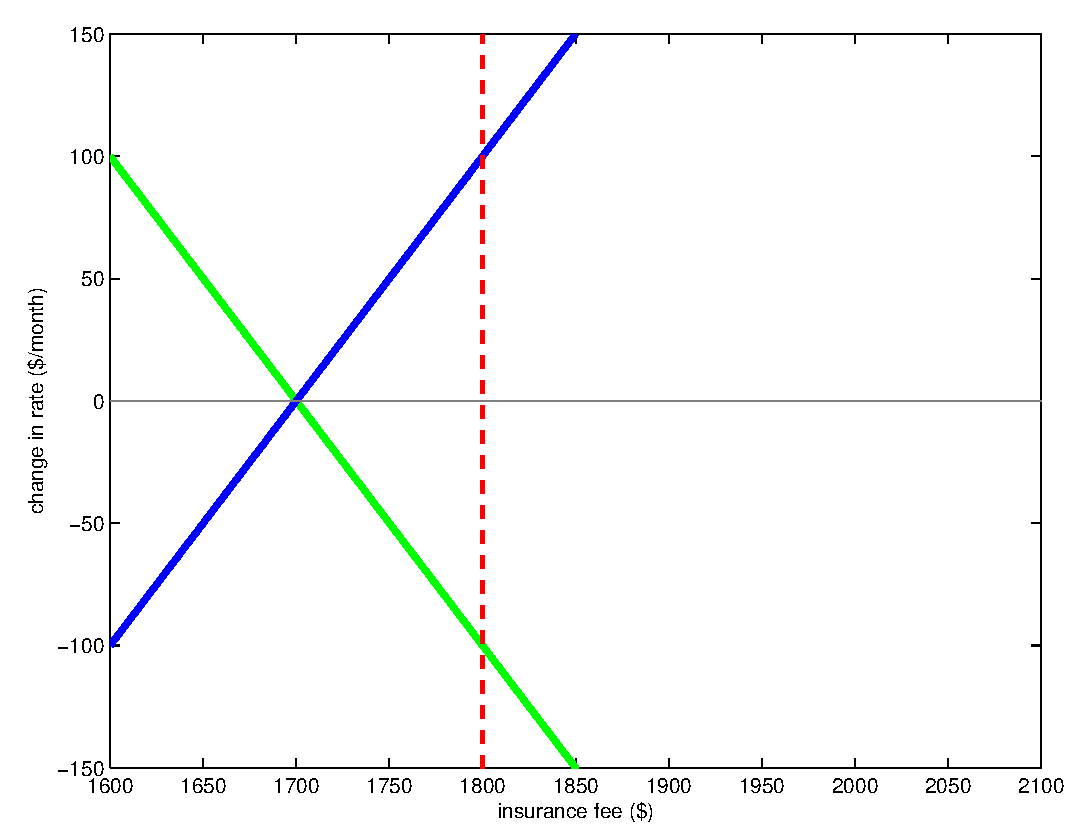
\includegraphics[width=0.9\textwidth]{./figs/ins_lin_cropped.pdf}
}

\frame{
\ft{Fix -- introduce asymmetry}
In this picture, the observed existence of insurance contracts requires some asymmetry between the parties:
\bi
\item different risk preferences;
\item different information about voyage;
\item different assessments of riskiness of voyage;
\item one party to deceive, coerce, gull other into bad decision.
\ei\mbox{}

Hard to accept as basis for large and important global market.
}

\frame{
\ft{Time paradigm}
\only<1>{
Resolve in time paradigm: assume multiplicative repetition and maximise $\gtm$.\np
Here multiplicative repetition means that owner sends ship and cargo whose values $\propto$ his wealth.\np
Rich owner sends more cargo in larger ship or flotilla, while poor owner sends small boat.\np
Under additive repetition, sends same cargo on each voyage, regardless of wealth.\np
Large shipping companies, \eg Maersk, inconceivable under additive repetition,
where profits not reinvested.
}
\only<2>{
Both parties seek to maximise their
\be
\gt_m = \lim_{\Dt\to\infty}\frac{\D\gv(\x)}{\Dt} = \frac{\ave{\d\ln \x}}{\dt}.
\ee
}
\only<3>{
Owner without insurance has 
\be
\gt_m^{(\text{o1})} = \frac{(1-\p)\ln(\x_\text{own}+\G)+\p\ln(\x_\text{own}-\C) - \ln(\x_\text{own})}{\dt}
\ee
or 1.9\% pm. Owner with insurance has
\be
\gt_m^{(\text{o2})} = \frac{\ln(\x_\text{own}+\G-\F)-\ln(\x_\text{own})}{\dt}
\ee
or 2.2\% pm. Difference is
\be
\d\gt_m^o = \gt_m^{(\text{o1})}-\gt_m^{(\text{o2})} \approx 0.24\% \text{ pm},
\ee
so owner signs contract in this world.
}
\only<4>{
An insurer who issues no insurance plays the null gamble:
\be
\gt_m^{(\text{i1})}= \frac{0}{\dt}
\ee
or 0\% pm. With insurance he has 
\be
\gt_m^{(\text{i2})} = \frac{(1-p)\ln(\x_\text{ins}+\F) + p\ln(\x_\text{ins}+\F-\gL) - \ln(\x_\text{ins})}{\dt}
\ee
or 0.0071\% pm. Difference is
\be
\delta\gbar_m^{\text{i}} = \gt_m^{(\text{i2})}-\gt_m^{(\text{i1})}\approx 0.0071\% \text{ pm},
\ee
so he is also keen to do business.
}
}

\frame{
\ft{Price range}
\centering
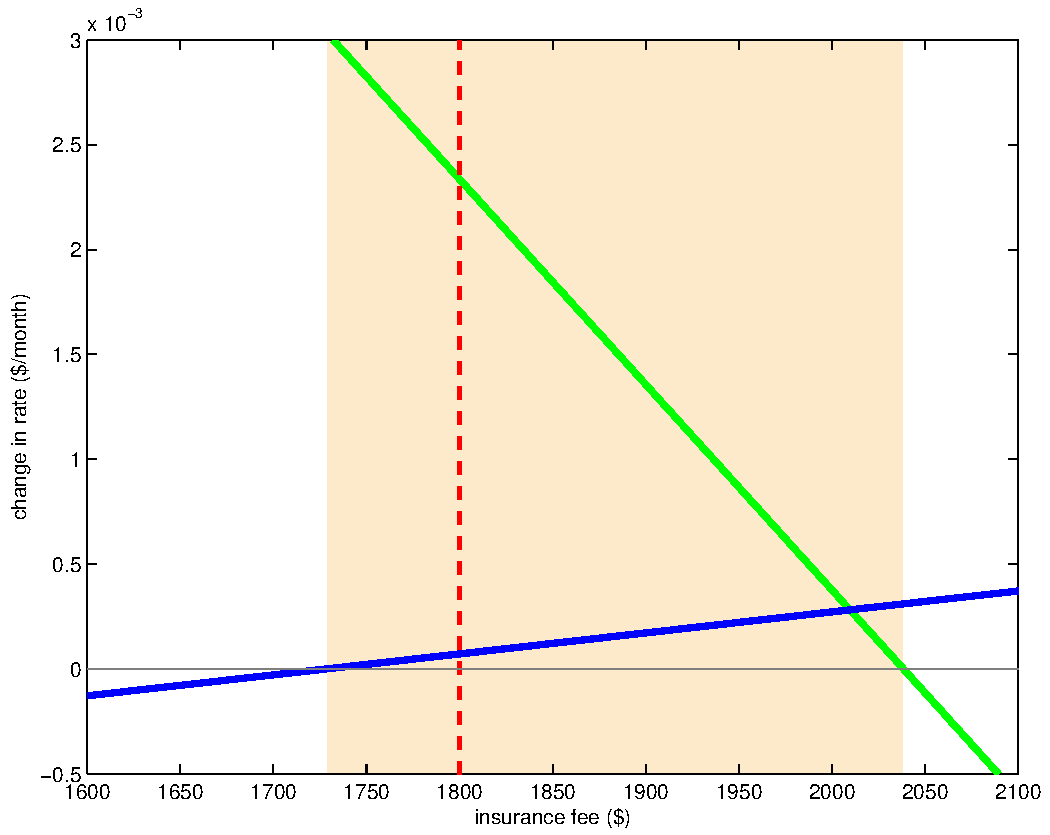
\includegraphics[width=0.9\textwidth]{./figs/ins_log_cropped.pdf}
}

\frame{
\ft{Fundamental resolution}
Time paradigm with multiplicative repetition creates a world where insurance contracts \textbf{can} exist.\np
We view this as the
\begin{keypts}{Fundamental resolution of the insurance puzzle:}
Buyer and seller of an insurance contract both sign when it increases the time-average growth rates of their wealths.
\end{keypts}\mbox{}

No appeal to asymmetries: arises naturally from our model of human decision-making.\np
\textit{Message: business happens when both parties gain.}
}

\end{document}